\toclesssection{SCP 014 - The Concrete Man}
\addcontentsline{toc}{section}{SCP 014 - The Concrete Man}

\fakebold{Item \#:} SCP-014

\fakebold{Object Class:} Safe

\begin{figure}[h]
\begin{center}
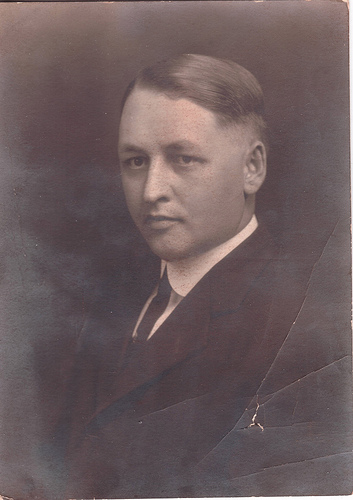
\includegraphics[scale=4]{scp/014.jpg}
\linebreak SCP-014 prior to initial confinement
\end{center}
\end{figure}

\fakebold{Special Containment Procedures:} SCP-014 is to be kept in Site-\censor{XX}, in a chair with arms, preferably facing a window. Music should be supplied on a regular basis, preferably constantly. This music should not include pieces originating after 1937. A security camera should be present in SCP-014's room.

\fakebold{Description:} SCP-014 is a Caucasian male, appearing to be approximately 30 years of age, with black hair, brown eyes, and a somewhat round face. Records indicate his name to be Robert Chetford, confined in 1915 to the Norwich Asylum in Connecticut for delusional insanity, claiming that he had been cursed to live forever, and was slowly turning into concrete in consequence. The asylum closed in 1937, and the patients were transferred to various other facilities. SCP-014 came to Foundation attention in 19\censor{XX}, from rumours of a patient who seemed to be entirely immobile and showed no signs of aging. Further investigation determined that acquisition was warranted.
\newpage
SCP-014 is to all outward appearances a normal man, but he does not appear to age, and shows no signs of possessing a metabolism. He does not eat, drink, perspire, or in any other way demonstrate life functions. He breathes only to speak, and apart from his eyes and vocal apparatus, is to all appearances utterly immobile. He has never shown any evidence of pressure ulcers despite his position not having varied for several decades; neither do his muscles appear atrophied. He can converse normally, but shows little knowledge of or interest in events since his confinement.

\fakebold{Addendum:}\linebreak
\textsl{Note: Frankly, were I to interview this man without knowing his history, I'd think he was a perfectly sane and well-adjusted individual who happens to be quadriplegic. As it is, I have to conclude that he's the ultimate proof of the idea that the mind rules the body. He thinks he's concrete, and will live forever, and so he's as close to both as he can be. Somehow. Dr. \censor{XXXXX}}